\section{Decision Trees}
\label{sec:dt}


\subsection{J48 Algorithm}
\label{sec:dt:j48}
\subsubsection{Variation in performance with size of the training and testing sets}
\raggedright\underline{Cross-Validation Accuracy On Different Files}


We executed the J48 Algorithm on fer2017-training/testing and fer2017-training/testing-happy using 10 fold cross validation. The full data set was used with the only variation being moving  9000 or 16000 from the training set to the testing set. This was done to see the effect of different sizes of training and testing set on the accuracy. The table below displays the data collected.

J48 is used to generate a decision tree. It is a supervised learning algorithm which requires a data set to be used as the training example. The algorithm analyses the training set and builds a classifier that can be used to correctly classify testing instances \autocite{octaviansima2013}. Some advantages are it is easy to implement and is easy to interpret. Some disadvantages are that the algorithm easily generalises and over fits to the training set. This is demonstrated by a small variation of data can lead to a different tree being constructed meaning that instead of training for the situation, it trains for the data in the training set.


\begin{figure}[hbt!]
	\centering
      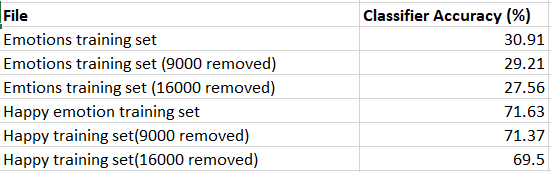
\includegraphics[width=0.7\textwidth]{imgs/J48/CVTraining.png} \\
	\caption{Cross validation accuracy on the training files}
	\label{fig:dt:CVTraining_table}
\end{figure}

Cross validation can be used to find out if the data set is overfitted to the training data, this will be discussed further in \ref{sec:dt:tts}. In figure \ref{fig:dt:CVTraining_table} the data displays that the accuracy of the J48 algorithm on training files with all emotion decreases from \textbf{`30.91\%'} to \textbf{`27.56\%'} when the data set is reduced incrementally. The computation time also decreased when the data set was reduced. The standard deviation of the training set on all emotions was relatively low apart from happy. 

Happy had both the highest TP and highest FP rate, this is due to Happy being the largest emotion in the data set. When observing the happy data, the effect of reducing the data set did not greatly impact the classifiers accuracy. The greatest difference is the set with 9000 thousand removed and the set of 16000 thousand removed decreasing from \textbf{`71.37\%'} to \textbf{`69.5\%'}.

\begin{figure}[hbt!]
	\centering
      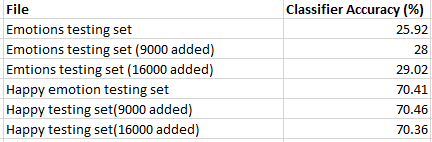
\includegraphics[width=0.7\textwidth]{imgs/J48/CVTesting.PNG} \\
	\caption{Cross validation accuracy on the testing files}
	\label{fig:dt:CVTesting_table}
\end{figure}


Cross validation being executed on the testing data sets displays the opposite when discussing the full emotion list compared to the training data. The accuracy increases from \textbf{`25.92\%'} to \textbf{`29.02\%'}. But the same remains when looking at the happy testing set with all tests concluding at around \textbf{`70\%'}.

\raggedright\underline\raggedright\underline{Testing on different test sets}

One of the main disadvantages of J48 is highlighted when testing on different test sets.

\begin{figure}[hbt!]
	\centering
      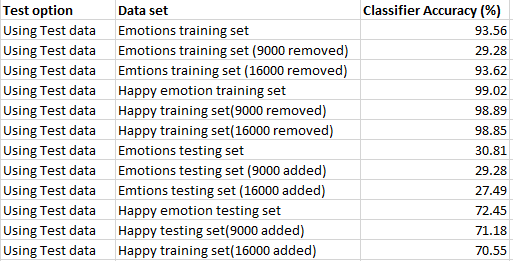
\includegraphics[width=0.7\textwidth]{imgs/J48/TestingOnDifferentTestSets.PNG} \\
	\caption{Accuracy using J48 on different test data}
	\label{fig:dt:Testingondifftests}
\end{figure}

Testing on unseen data, the test data-sets, J48 has low classifier accuracy relatively similar to the accuracy found in cross validation. All emotions with all rows had \textbf{'30.81\%'} dropping off to \textbf{'27\%' }when 16000 more rows were added to the testing set. This demonstrates J48's flaws in generalising and over-fitting to the training set. This is further demonstrated when the algorithm passed the same file for the training set and the testing set. In the instance of all emotions with all rows it produces a correctly classified accuracy of \textbf{93.56\%} which displays its over-fitting to the training set, compared to the \textbf{30.81\%} when given new unseen testing data. The standard deviation of the TP rates in this example is relatively small, this seems to be the trend across all of the data. 


\subsubsection{Variation in performance with varying learning parameters in J48 algorithm}

Several parameters were changed to study the effect they would have on the J48 algorithm.

\begin{enumerate}
\item Binary splits was used on each test. Binary split is a process which the tree is grown by considering different nominal values verses each other instead of considering a sl
https://www.schankacademy.com/demos/data-analytics/xt/lib/docs/0/j48\_parameters.pdf
\end{enumerate}


\raggedright\underline{Variation in performance according to different metrics}



\subsection{Random Forest}
\label{sec:dt:rf}
For this coursework we had to select one other decision tree algorithm. The algorithm we decided to use was the Random Forest algorithm \autocite{Breiman2001}. This was selected due to the coursework's focus on overfitting. The Random Forest algorithm helps to fix the overfitting that J48 is prone to. The complexity of a classifier such as J48 can reach a point where it is negatively impacted by overfitting. The nature of Random Forest algorithm means that increased iterations do not lead to a point where it is perfectly optimised for the training set and therefore harming the accuracy of the testing set. Machine Learning algorithms should be well optimised for unseen test data, rather than training data. The algorithm in WEKA is based on Breiman's implementation \autocite{Breiman2001}. It combines bagging with a random selection of features. Bagging combines the classifications of randomly generated subsets of the main training set. Random selection of features further reduces overfitting by allowing the algorithm to only select a set number of randomly chosen features. Each iteration in WEKA produces a new decision tree. An instance(row) in the data set is classified by finding the mode class of all the trees. For example, if you have 10 iterations there will be 10 decision trees. If 6 trees classify the pixel attributes as Happy then it will be classified as happy because it is the highest mode. We discovered that random forest consistently performed better than J48 with quicker compile time.

Using Python we automated numerous different experiments, totalling 688 executions of the algorithm on different testing options and parameters. These results are summarised in 6 tables found in the Appendix (section 5.3.1). We ran the algorithm on 16 different test options. The required ones were crossfold on the training set and using the test sets with varying number of instances (totalling 8 different test options). I additionally ran crossfold on the test set (smaller data comparison) and used the training sets as a test set (to use in discussion of overfitting). Below is a summary of the analysis found.  

\raggedright\underline{Variation in performance with size of the training and testing sets}

\begin{enumerate}
  \item Larger data sets perform better. The classifier accuracy using crossfold on the original training set (28709 instances) was consistently higher than the original test set (7178 instances). This was true for both Happy and All emotions. 10 crossfold validation on Happy Training set produced 78.24\% accuracy whereas on the Test set it produced 76.95\%. The Emotions data saw a much larger decrease in accuracy when using the test set dropping from 44.25\%(training set) to 37.57\%(test set). An increase in data improves the training of the random forest algorithm.
  \item Using the test set rather than crossfold validation produces higher accuracy. This is expected as crossfold validation gives a more realistic measure of how well a model will classifier unseen data.
  \item Moving instances from the training set to the test set reduces accuracy in both Happy and all emotions data set. This is expected as the classifier has less data to build a model which will be tested on more data. More instances in the test data means more cases for the model to handle. Logically, the more cases a model has to handle the lower the chance of classification. Furthermore, the change in ratio of training to test data means that after adding 16000 instances to the test set you are in fact using a test set that is larger than the data used to train. The significance of this is that smaller training set will be prone to more bias. This model with increased bias towards the training data is now tested on a larger quantity of data with did not impact the bias. The decrease in accuracy is supported by the results. Using the original test set the classifier built on emotions training data produced 45.56\%. Moving 9000 instances to the test set saw a drop to 43.42\% and 16000 saw a further drop to 40.11\%. This pattern was the same for the Happy test set. The original version had accuracy of 78.75\%. The test set with 9000 instances added was 77.91\% and with 16000 added it was 77.53\%. Interestingly it saw a smaller drop in accuracy than all emotions. This is likely due to the fact that it only has to learn to classify between two nominal values rather than seven. Overall, the fall in accuracy suggests that the Random Forest algorithm needs both a large amount of data and large ratio of data in comparison  the test set to more accurately classify. 
  \item Using the training sets for testing consistently produces accuracy close to 99\%. This is not necessarily a good thing as it means the model is very optimised for the training data when it should be optimised for unseen data. High accuracy is expected as it is not testing on unseen data. 
\end{enumerate}


\raggedright\underline{Variation in performance with varying learning parameters in Random Forest}

The parameters for Random Forest we experimented with was: starting seed, number of iterations, max depth, number of features and bag size. This section summarises our findings.
\begin{enumerate}
    \item The starting seed is pseudo-randomisation which gives you the ability to repeat experiments. In an ideal world this will not have a big impact on accuracy. This will of course affect the "random" aspect of the random forest and as such the starting seed produced different accuracy. We tested starting seed 1 to 10 and found that generally the accuracy did not vary more than 1\%. This is positive because out of all parameters tested this is the one that ideally would vary the least in accuracy. The most noticeable exception to this generalisation was the impact it had when using the original emotions test set. The accuracy varied from between 44.45\% to 46.48\%, a significant different of 2.03\%. The starting seed should be taken into consideration when using random forest, but it should not be the focus when trying to optimise.
    \item Our next experiment was the number of iterations, we tested between 10 iterations and 150. Each iteration generates a new decision tree, 10 iterations means 10 trees etc. The number of iterations had a far greater impact on the emotions data set classifier accuracy than it did on the Happy data set. The pattern for both data sets was that more iterations meant increased accuracy up to a certain point; emotions saw a far bigger increase than happy. Doing 10 iterations on the emotions data using crossfold validation with the emotions training data had an accuracy of 35.57\%. It continuously rose up with the increase in iterations, 150 iterations had an accuracy of 44.95\% by comparison. A large number of iterations is needed to encompass the emotions data set. Happy did not exhibit the same behaviour. Increasing iterations using the same test options (with Happy data) actually peaked at 90 iteration with accuracy of 78.29\%. The classifier may be overfitting after 90 iterations. The number of iterations has a big impact on performance, increasing the number of iterations will improve accuracy up to an optimum point. This is true for all testing options. 
    \item Bag Size Percent affected the accuracy. It is 100\% by default, so we tested 5\%, 10\%, 15\% and 50\%. A smaller bag size (smaller percentage of the data-set) caused the accuracy to go down. Each decrease in bag size percentage negatively affected the classifier. This is because it is modelling with a smaller percentage of the data set. Its main benefit was increased compile time. 
    \item Our next experiment was varying the number of features the algorithm had to choose between. The default in WEKA is log2(number of attributes)+1, which for the emotions data set is log2(2304)+1 which is approximately 12. We discovered that increasing the number of features the algorithm had to choose between increased the accuracy for all test options. A larger range of features to choose between allows a classifier to better represent the problem. The default option does not optimise the number of features. The largest increase was when using the Happy test set with 9000 instances. Number of features set to 5 produced 76.98\% whereas number of features set to 100 produced 79.8\%. Increasing the number of features improved accuracy but there may be a computational benefit to setting number of features to a lower number. Setting number of features from 5 to 100 improved the accuracy at most by 2.82\%.
    \item Finally, we looked at setting the max depth of the tree. We had a theory that setting a max depth may help to reduce overfitting because the tree is limited to how well it can fit the training set. We were not able to confirm this theory because the largest max depth (10) we tested produced the best accuracy across all test options. There may be a max depth limit beyond this which restricts and optimises the tree on test set, but further experimentation is needed to discover this. Increasing max depth from 3 to 10 improved accuracy across all test options. The appendix shows these improvements. One thing to note is that the max depth had the biggest impact on the accuracy of the classifier when using the training set for testing. The accuracy of using the test set and training set for testing is in fact very similar up to max depth up to max depth 6. Max depth 7 and above clearly does a better job of fitting to the training set. 
\end{enumerate}


\raggedright\underline{Variation in performance according to different metrics }

The section on Random Forest is already extensive, so I will mention the most noticeable/interesting metrics. 










\subsection{User Classifiers}
\label{sec:dt:uc}
After running the \textbf{Random Forest} experiments we constructed a semi-manual tree with the \textbf{500, 1000, 1250, 1500 and 2000} pixel attributes selected to perform binary splits on the \textbf{emotions test set.} This then had the \textbf{Random Forest} classifier applied to the leaf node as seen in \textbf{figure \ref{fig:dt:semi_manual_random_forrest}}. We applied this to the non-split training and testing data, using the `\textbf{Supplied test set}' option, as well as the `\textbf{Cross-validation}' with 10 folds specified. The settings used for the classifier in the semi-manual tree is shown in \textbf{figure \ref{fig:appendix:classifier:rfucs}} at \textbf{appendix \ref{sec:appendix:classifier:rfucs}} and is the default settings for \textbf{Random Forest}.

\begin{figure}[hbt!]
	\centering
      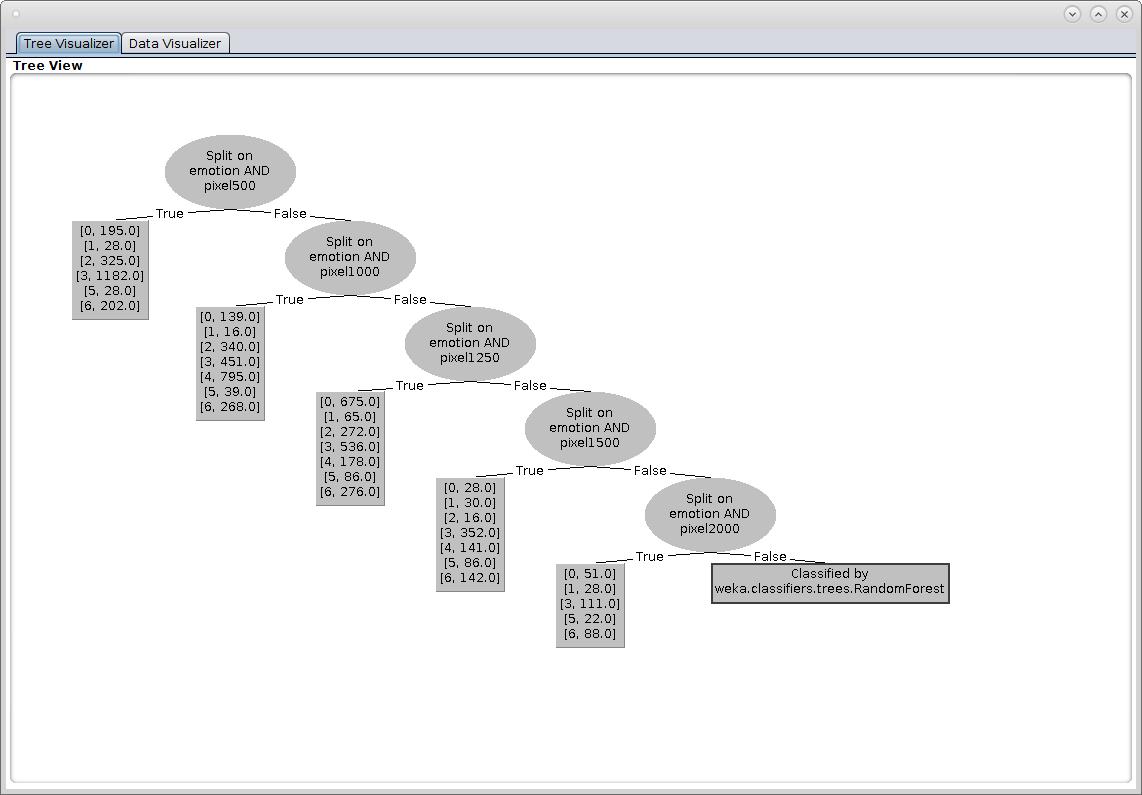
\includegraphics[width=0.6\textwidth]{imgs/userClassifier/noSplit/all/Train-and-Test/tree_settings_with_classifier.png} \\
	\caption{Semi-Manual Tree with Random Forrest Classifier}
	\label{fig:dt:semi_manual_random_forrest}
\end{figure}


When selecting points to be removed from our chosen pixels we aimed to select edge cases, where data points appear as \textit{anomalies}. This focused the data into larger clumps, narrowing an emotion's correlation with the pixel values. Looking at \textbf{figure \ref{fig:dt:supplied_test_set:pixel500},}  red emotion \textbf{Disgust (1)} highlights value points which were sparsely grouped at the top and bottom of the pixel value range. This was done consistently with each emotion on the specified pixels \textbf{500, 1000, 1250, 1500 and 2000}. 

\FloatBarrier
\begin{figure}[hbt!]
	\centering
      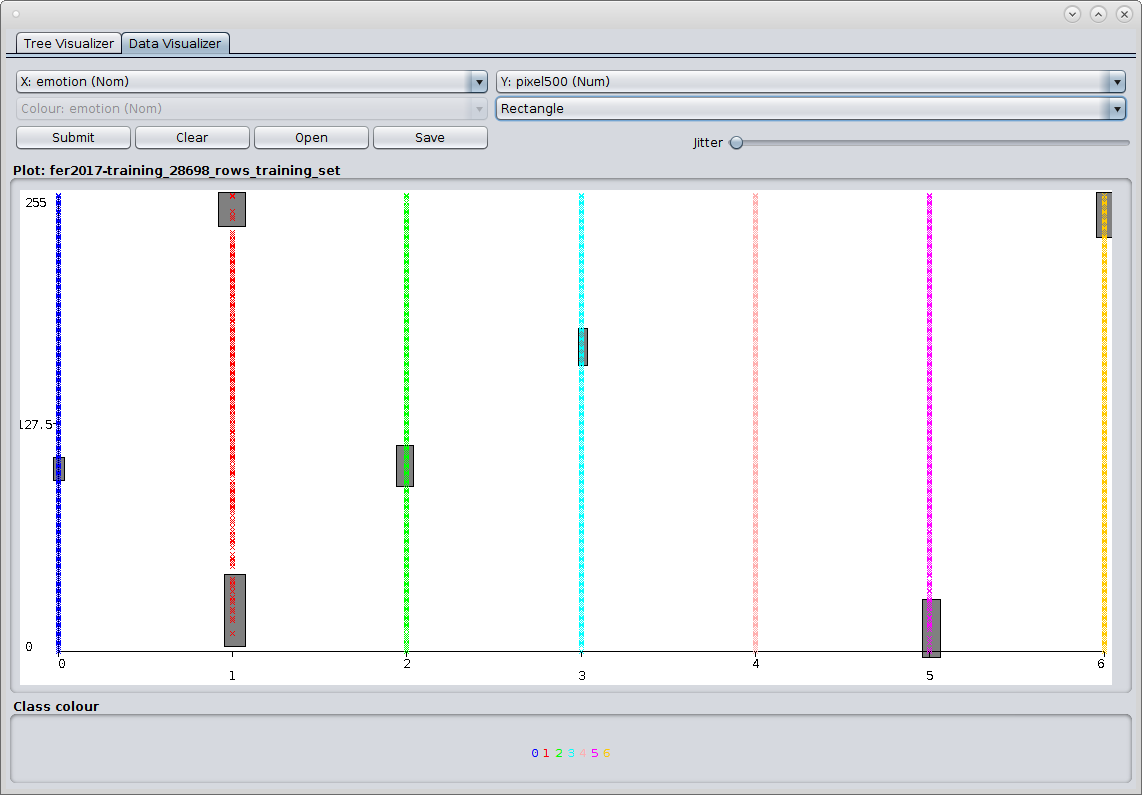
\includegraphics[width=0.6\textwidth]{imgs/userClassifier/noSplit/all/Train-and-Test/500.png} \\
	\caption{Pixel 500 Selected Pixel Values}
	\label{fig:dt:supplied_test_set:pixel500}
\end{figure}

Our results produced from both of these experiments can be seen in \textbf{figure \ref{fig:dt:uc:results}}, with \textbf{cross-validation} producing a lower classifier accuracy of \textbf{39.19\%} compared to  \textbf{supplied test set} producing a slightly higher \textbf{42.59\%}. These results of cross-validation reducing the over-fitting of data is consistent with our findings in \textbf{section \ref{sec:dt:rf}} above. 

\FloatBarrier
\begin{figure}[hbt!]
	\centering
      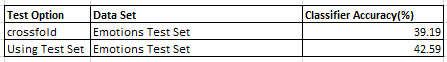
\includegraphics[width=0.75\textwidth]{imgs/userClassifier/noSplit/all/userclassifier_accuracy_results.PNG} \\
	\caption{Cross-validation and Using test set results with User Classifiers and Random Forest}
	\label{fig:dt:uc:results}
\end{figure}

\subsubsection{Supplied Test Set}
\label{sec:dt:uc:sts}

Building the classifier with \textbf{fer2017-training\_28698\_rows\_training\_set.arff} and supplying test data with \textbf{fer2017-testing\_rows\_testing\_set.arff} produced an accuracy of \textbf{42.59\%} (\textbf{Figure \ref{fig:dt:uc:results}}) compared to \textbf{45.56\%} from the default \textbf{Random Forest} experiment with the same input data (\textbf{Appendix \ref{sec:appendix:charts_tables}, figure \ref{fig:randomforest_main}}). The \textit{FP} rates are consistently higher for the User Classifier Random Forest (\textbf{UC Random Forest}) compared to the default classifier of the \textbf{Random Forest} algorithm. The only exception of this can be seen for the \textbf{Happy (3)} emotion which has a higher \textit{FP} rate at\textit{ 0.364} compared to \textit{0.233} (\textbf{Table \ref{table:uc:randForest_vs_UCrandForest_tpfp}}). This is appears due to \textbf{Random Forest} predicting \textbf{TP} rates that match closely to the ratio of distribution of emotions in the file, whereas \textbf{UC Random Forest} is predicting emotions over a broader range of the data-set, shown by a smaller standard deviation of the \textit{FP} values. This shows that \textbf{UC Random Forest} is predicting more inaccurately, and shows the importance of edge cases of the emotion's data values. \textbf{UC Random Forest} performs slightly worse due to user intervention of selecting pixels to discard than simply applying \textbf{Random Forest} to the whole data-set. 

\FloatBarrier
\begin{table}[htb!]
\begin{center}
 \begin{tabular}{||P{0.105\linewidth}|P{0.1\linewidth}|P{0.1\linewidth}|P{0.1\linewidth}|P{0.1\linewidth}|P{0.1\linewidth}|P{0.1\linewidth}|P{0.1\linewidth}||} 
 \hline
 \textbf{TP}-\textit{FP} Rates 
 & \textbf{Angry (0)} 
 & \textbf{Disgust (1)} 
 & \textbf{Fear (2)} 
 & \textbf{Happy (3)} 
 & \textbf{Sad (4)} 
 & \textbf{Surprise (5)} 
 & \textbf{Neutral (6)} 
 
 \\ \hline\hline
 
 \textbf{Random Forest} 
 & \textbf{0.193}-\textit{0.037} 
 & \textbf{0.318}-\textit{0.0} 
 & \textbf{0.259}-\textit{0.046} 
 & \textbf{0.804}-\textit{0.364} 
 & \textbf{0.335}-\textit{0.106} 
 & \textbf{0.602}-\textit{0.033} 
 & \textbf{0.356}-\textit{0.099}
 
 \\  \hline
 
 \textbf{UC Random Forest} 
 & \textbf{0.18}-\textit{0.039} 
 & \textbf{0.255}-\textit{0.0} 
 & \textbf{0.289}-\textit{0.087} 
 & \textbf{0.625}-\textit{0.233} 
 & \textbf{0.352}-\textit{0.129} 
 & \textbf{0.645}-\textit{0.066} 
 & \textbf{0.387}-\textit{0.151}
 
 \\ \hline
 
 \hline
\end{tabular}
\caption{Random Forest vs. User Classifier Random Forest \textbf{TP}-\textit{FP} Rates}
\label{table:uc:randForest_vs_UCrandForest_tpfp}
\end{center}
\end{table}



\FloatBarrier
\subsubsection{Crossfold-Validation}
\label{sec:dt:uc:cfv}
Applying \textbf{fer2017-training\_28698\_rows\_training\_set.arff} to crossfold-validation produced an accuracy of 39.19\% (\textbf{Figure \ref{fig:dt:uc:results}}) compared to 44.25\%  from the default \textbf{Random Forest} experiment with the same input data (\textbf{Appendix \ref{sec:appendix:charts_tables}, figure \ref{fig:randomforest_main}}). Consistent with the evaluation in section \ref{sec:dt:uc:sts}, \textbf{UC Random Forest} has a smaller standard deviation over the emotions \textbf{TP} and \textit{FP} rates compared to \textbf{Random Forest} in table \ref{table:uc:CROSSFOLD_randForest_vs_UCrandForest_tpfp} which does not accurately represent the ratio of emotions distributed in the file.  Furthermore, it has more higher \textit{FP} and lower \textbf{TP} rates compared to \textbf{Random Forest}, bar the \textbf{Happy (3)} emotion, suggesting the \textbf{UC Random Forest} is more varied and less accurate than the standard \textbf{Random Forest}.


\FloatBarrier
\begin{table}[htb!]
\begin{center}
 \begin{tabular}{||P{0.105\linewidth}|P{0.1\linewidth}|P{0.1\linewidth}|P{0.1\linewidth}|P{0.1\linewidth}|P{0.1\linewidth}|P{0.1\linewidth}|P{0.1\linewidth}||} 
 \hline
 \textbf{TP}-\textit{FP} Rates 
 & \textbf{Angry (0)} 
 & \textbf{Disgust (1)} 
 & \textbf{Fear (2)} 
 & \textbf{Happy (3)} 
 & \textbf{Sad (4)} 
 & \textbf{Surprise (5)} 
 & \textbf{Neutral (6)} 
 
 \\ \hline\hline
 
 \textbf{Random Forest} 
 & \textbf{0.197}-\textit{0.034} 
 & \textbf{0.245}-\textit{0.0} 
 & \textbf{0.257}-\textit{0.047} 
 & \textbf{0.794}-\textit{0.381} 
 & \textbf{0.319}-\textit{0.111} 
 & \textbf{0.558}-\textit{0.035} 
 & \textbf{0.345}-\textit{0.096}
 
 \\  \hline
 
 \textbf{UC Random Forest} 
 & \textbf{0.2}-\textit{0.06} 
 & \textbf{0.151}-\textit{0.0} 
 & \textbf{0.233}-\textit{0.063} 
 & \textbf{0.584}-\textit{0.251} 
 & \textbf{0.273}-\textit{0.112} 
 & \textbf{0.479}-\textit{0.046} 
 & \textbf{0.48}-\textit{0.218}
 
 \\ \hline
 
 \hline
\end{tabular}
\caption{Crossfold Random Forest vs. User Classifier Random Forest \textbf{TP}-\textit{FP} Rates}
\label{table:uc:CROSSFOLD_randForest_vs_UCrandForest_tpfp}
\end{center}
\end{table}



\FloatBarrier